\documentclass[mgr, oneside, en]{mgr}
\usepackage{listingsutf8}

\usepackage{booktabs, multirow} % for borders and merged ranges
\usepackage{soul}% for underlines
\usepackage[table]{xcolor} % for cell colors
\usepackage{changepage,threeparttable} % for wide tables

\usepackage[english]{babel}
\usepackage[utf8]{inputenc}
\usepackage[T1]{fontenc}
\usepackage[ruled,vlined]{algorithm2e}

\usepackage{graphicx}
\usepackage{subfigure}
\usepackage{psfrag}

\usepackage{amsmath}
\usepackage{amsfonts}

\usepackage{supertabular}
\usepackage{array}
\usepackage{tabularx}
\usepackage{hhline}

\usepackage{listings}
\usepackage{rotating}
\usepackage{graphicx}
\usepackage{setspace}
\usepackage{caption}
\usepackage{float}
\usepackage{placeins}

\usepackage[utf8]{inputenc}
\usepackage[acronym]{glossaries}


\makenoidxglossaries

% TODO use all acronyms

\newacronym{pg}{PG}{PostgreSQL}
\newacronym{vu}{VU}{Virtual User}
% \newacronym{orm}{ORM}{Object-Relational Mapping}
\newacronym{mvc}{MVC}{Model-View-Controller}
\newacronym{wsgi}{WSGI}{Web Server Gateway Interface}
\newacronym{asgi}{ASGI}{Asynchronous Server Gateway Interface}
\newacronym{npm}{NPM}{Node Package Manager}
% \newacronym{js}{JS}{JavaScript}
\newacronym{crud}{CRUD}{Create Retrieve Update Delete}
\newacronym{http}{HTTP}{Hypertext Transfer Protocol}
\newacronym{api}{API}{Application Programming Interface}


\renewcommand{\labelenumii}{\theenumii}
\renewcommand{\theenumii}{\theenumi.\arabic{enumii}.}

\newfloat{pseudocode}{thp}{lop}[chapter]
\floatname{pseudocode}{Pseudokod}

\usepackage{listingsutf8}
\usepackage{xcolor}

\lstdefinelanguage{docker}
{
    keywords={FROM, RUN, COPY, ADD, ENTRYPOINT, CMD,  ENV, ARG, WORKDIR, EXPOSE, LABEL, USER, VOLUME, STOPSIGNAL, ONBUILD, MAINTAINER},
    keywordstyle=\color{blue},
    identifierstyle=\color{black},
    sensitive=false,
    comment=[l]{\#},
    commentstyle=\color{magenta}\ttfamily,
    stringstyle=\color{red}\ttfamily,
    morestring=[b]',
    morestring=[b]"
}

\lstdefinelanguage{docker-compose}
{
    keywords={image, environment, ports, container_name, ports, volumes, links},
    keywordstyle=\color{blue}\bfseries,
    identifierstyle=\color{black},
    sensitive=false,
    comment=[l]{\#},
    commentstyle=\color{magenta}\ttfamily,
    stringstyle=\color{red}\ttfamily,
    morestring=[b]',
    morestring=[b]"
}
\lstdefinelanguage{docker-compose-2}{
    keywords={version, services},
    keywordstyle=\color{cyan}\bfseries,
    keywords=[2]{image, environment, ports, container_name, ports, links, build, volumes, depends_on, env_file, stdin_open, tty, profiles, mem_reservation, condition, healthcheck, test, interval, timeout, retries},
    keywordstyle=[2]\color{blue}\bfseries,
    identifierstyle=\color{black},
    sensitive=false,
    comment=[l]{\#},
    commentstyle=\color{magenta}\ttfamily,
    stringstyle=\color{red}\ttfamily,
    morestring=[b]',
    morestring=[b]"
}

\lstset{
    basicstyle=\ttfamily,
    showstringspaces=false,
    commentstyle=\color{red},
    keywordstyle=\color{blue},
    inputencoding=utf8,
    extendedchars=true
}
\definecolor{lightgray}{rgb}{.9,.9,.9}
\definecolor{darkgray}{rgb}{.4,.4,.4}
\definecolor{purple}{rgb}{0.65, 0.12, 0.82}

\lstdefinelanguage{JavaScript}{
    keywords={typeof, new, true, false, catch, function, return, null, catch, switch, var, if, in, while, do, else, case, break, const},
    keywordstyle=\color{blue}\bfseries,
    ndkeywords={class, export, boolean, throw, implements, import, this, async, require},
    ndkeywordstyle=\color{darkgray}\bfseries,
    identifierstyle=\color{black},
    sensitive=false,
    comment=[l]{//},
    morecomment=[s]{/*}{*/},
    commentstyle=\color{purple}\ttfamily,
    stringstyle=\color{red}\ttfamily,
    morestring=[b]',
    morestring=[b]",
    morestring=[b]`,
}

\lstset{
    language=JavaScript,
    %   backgroundcolor=\color{lightgray},
    extendedchars=true,
    basicstyle=\footnotesize\ttfamily,
    showstringspaces=false,
    showspaces=false,
    %   numbers=left,
    %   numberstyle=\footnotesize,
    %   numbersep=9pt,
    tabsize=2,
    breaklines=true,
    showtabs=false,
    captionpos=b
}


%pakiet wypisujący na marginesie etykiety równań i rysunków zdefiniowanych przez \label{}, chcąc wygenerować finalną wersję dokumentu wystarczy usunąć poniższą linię
% \usepackage{showlabels}

%definicje własnych poleceń
\newcommand{\R}{I\!\!R} %symbol liczb rzeczywistych, działa tylko w trybie matematycznym
\newtheorem{theorem}{Twierdzenie}[section] %nowe otoczenie do składania twierdzeń
\renewcommand\lstlistlistingname{List of Code Listings}

% STRONA TYTULOWA
\title{Analiza porównawcza i ocena wydajności frameworków back-endowych w
aplikacjach bazodanowych}
\engtitle{Comparison analysis and efficiency evaluation of back-end frameworks in
database applications}
\author{Marcin Wojciechowski}
\supervisor{Dr inż. Paweł Głuchowski W4/K30}
%\guardian{Dr inż. Paweł Trajdos} %nie używać jeśli opiekun jest tą samą osobą co prowadzący pracę

\date{2021}

\field{Informatyka Techniczna (INF)} % TODO find INF english name

\specialisation{Internet Engineering (INE)}

\begin{document}
\bibliographystyle{ieeetr}
\maketitle

% DEDYKACJA
% \dedication{6cm}{To jest przykładowa treść opcjonalnej dedykacji, należy ją zmienić lub usunąć w całości polecenie \texttt{$\backslash$dedication}}

\setcounter{tocdepth}{1}
\tableofcontents

%
%
% TRESC PRACY
%
%

\addcontentsline{toc}{chapter}{Acronyms and abbreviations}
\printnoidxglossary[type=\acronymtype, title=Acronyms and abbreviations, toctitle=List of Acronyms and abbreviations]

% !TeX root = ./0Base.tex

\chapter{Introduction}

Complex web applications keep becoming more popular in recent years. They are very easily accessible from any place in the world and can run on almost any modern device, as it requires only web browser and the Internet connection to run.

Web frameworks simplify the development process of web applications significantly improving developers productivity. There is a huge variety of choices between the mentioned software, so choosing one may be a difficult task.

The choice of server-side framework is crucial, as it is responsible for handling sensitive data and plays a key role in the overall performance of the application.

The goal of this document is to focus on three of the most popular server-side frameworks and compare their performance under high load as well as basic security measurements. The results of this thesis will be important for web developers and architects, that need to decide on which framework should they choose for their application.

Web frameworks for this comparison were chosen from the list of Stack Overflow Developer Survey 2020 Web Frameworks popularity \cite{devSurvey}. The chosen frameworks (and their respective languages) are:
\begin{itemize}
    \item Express.js (JavaScript)
    \item ASP.NET (C\#)
    \item Django (Python)
\end{itemize}

Chapter 2 describes chosen frameworks, including their architecture and requirements. For the definition of the criteria against which the results will be measured, see Chapter 3. Chapter 4 presents design of the system - database models, application structure and environment preparation. Chapter 5 shows framework specific application implementation details. Results of the tests and comparison of the technologies can be found in chapter 6. For final conclusion of this document, see chapter 7.


% !TeX root = ./0Base.tex

\chapter{Technology description}

\section{Django}

\subsection{Overview}
Django lets you build deep, dynamic, interesting sites in an extremely short time. Django is designed to let you focus on the fun, interesting parts of your job while easing the pain of the repetitive bits \cite{djangobook}. Additionally the framework is being supported by a wide variety of libraries and frameworks, like Django Rest Framework, Django Celery, Crispy Forms.

\subsection{Architecture}
Django is based on MVC architecture:
\begin{itemize}
    \item Model - a data structure, represented by a database
    \item View - responses visible in the browser
    \item Controller - connects Model and View together - describes how the data should be presented to the user
\end{itemize}
In Django application there are multiple files and at first it may not be obvious what their role is. Basic structure looks like this:
\begin{itemize}
    \item apps.py - common to all django apps configuration file
    \item models.py - custom models
    \item serializers.py - define how our model objects should be converted into response
    \item views.py - custom controllers, which is unintuitive for most of people; as the developers explain, in their interpretation of MVC the view describes which data gets presented to the user \cite{djangoWhyViews}
    \item urls.py - defines which endpoint responds to given controller
\end{itemize}
Templates, which are not mentioned above, are the Django's custom views - in our case, I am going to be using build in json parsers.

\subsection{Requirements}
To install and run a simple Django project, two main things are required:
\begin{itemize}
    \item pip (easiest install method)
    \item Python
\end{itemize}


\section{ExpressJS}

\subsection{Overview}
\subsection{Architecture}
\subsection{Requirements}


\section{ASP.NET}

\subsection{Overview}
\subsection{Architecture}
\subsection{Requirements}

\section{K6 and related tools}

For testing the performance of applications, I chose a tool named k6. It is a modern load testing tool written in Golang, which provides clean and well documented APIs for writing and running tests, while still being easily configurable to the developers needs. Test logic and configuration options are both to be written in JavaScript, which allows developers for using JavaScript modules, which aids in code reusability. The creators of k6 prepared two types of execution:
\begin{itemize}
    \item local, through command line interface
    \item and cloud, which is a commercial SaaS product, made to make performance testing in bigger applications easier.
\end{itemize}
For the sake of this experiment, local testing has fulfilled all expectations.

Installation on Ubuntu operating system is fairly simple and all necessary commands were described in the documentation. However, to make the testing simpler, a k6 Docker image was used, that together with Docker Compose allowed to create a single script that would handle all test cases as described in the following section.

K6 allows to create visualizations, using built-in InfluxDB and Grafana integration, where InfluxDB is used as storage backend and Grafana to visualize the data. In this research, only InfluxDB was added to store the data and after each test the data was exported to file, which later allowed to compare the results between applications on a single chart.

\section{Docker and Docker Compose}

Docker and Docker Compose were used to simplify the development. This made starting all services that had be run together possible with only one command, eg. for django performance tests - django, postgres, k6 and influx. For every application a production ready Dockerfile was created. Additionally, Docker provides applications a layer of isolation from each other and the host.

\section{PostgreSQL}

For the Database Management System I chose PostgreSQL, which is the second most popular choice among database technologies %TODO link to dev survey


% !TeX root = ./0Base.tex

\chapter{Criteria description}

\section{Performance benchmark}

\subsection{Scenarios}
The task for each application is to complete simple \acrshort{crud} operations as fast as possible. For comparison of the performance of the applications, a few test cases were developed:

\begin{itemize}
    \item retrieving multiple objects (getMany)
    \item retrieving single object (get)
    \item updating a single object (put)
    \item creating a single object (post)
    \item deleting a single object (delete)
\end{itemize}

They were tested with a few different application loads, which are represented by a number of \acrlong{vu}s (\acrshort{vu}s) - as mentioned in the k6 repository description they are glorified, parallel while(true) loops.
% TODO ref to k6 repo
The scenarios chosen for tests are:
\begin{itemize}
    \item 1 \acrshort{vu}
    \item 8 \acrshort{vu}s
    \item 32 \acrshort{vu}s
    \item 128 \acrshort{vu}s
    \item 512 \acrshort{vu}s
\end{itemize}
For a single virtual user case the number of concurrences does not change throughout the duration of the test, however, as suggested in
% TODO find article that suggests this
, for bigger numbers of concurrent users, the tests should include warmup and cooldown period. All tests are 45 seconds long, and tests with more than 1 virtual user include 15 seconds of ramp up time and 15 seconds of ramp down time as shown on figure \ref{fig:vusPerSecond}.

Longer test times did not bring any satisfactory results and only caused CPU throttling problems, thus they were shortened to the period of 45 total seconds, which also made comparison of the results much easier.

For one scenario the results could be slightly different, that is why every test was repeated 10 times. For creation of the graphs presented in chapter \ref{chapter:7} for each test an average response times were calculated. % TODO ref chapter 7 

\begin{figure}[H]
    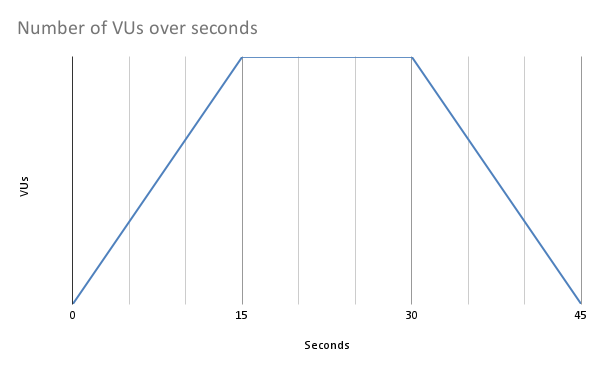
\includegraphics[width=\columnwidth]{pictures/vusPerSecond.png}
    \caption{Amount of VUs per second during the tests}
    \label{fig:vusPerSecond}
\end{figure}


\subsection{Data}

For the performance tests some frameworks required initial data to exist in the database (for example PUT endpoint for editing database models), thus at the beginning of the tests for each framework the database is populated. To be sure that the data is consistent, after seeding the database the docker volume that keeps the data is being stored locally, and before each test it is being restored.

\subsection{Application isolation}

To be sure that the applications are running in an isolated environment, docker containers were used. The configuration prepared for the applications included environment preparation (installing necessary packages, providing environment variables), To simplify the research, a Docker Compose configuration was prepared, that builds and starts all the necessary containers at once.

\subsection{Test progress}

The main script prepared for this thesis, that gathers all the measurements is described in the algorithm \ref{alg:testProgress}.

\begin{algorithm}[H]
    \label{alg:testProgress}
    \caption{Pseudocode describing load testing process}

    frameworks = [aspnet django express]\;
    scenarios = [1 8 32 128 512]\;
    iterations = [1 2 3 4 5 6 7 8 9 10]\;
    test cases = [get post put delete getMany]\;

    \ForAll{frameworks}{
        start application and database\;
        populate database\;
        kill application and database\;
        store snapshot\;
        \ForAll{scenarios}{
            \ForAll{iterations}{
                \ForAll{test cases}{
                    \If{application is running}{kill application and database\;}
                    remove volumes\;
                    \If{test case is not post}{restore snapshot\;}
                    start application and database\;
                    \While{application is not responding}{wait for application\;}
                    \For{45 seconds}{measured test\;}
                    store k6 result \;
                    store influxDB result \;
                    \For{20 seconds}{cooldown before next test\;}
                }
            }
        }
    }
    merge results\;
\end{algorithm}


\subsection{Software versions and hardware}

The tests were run on a laptop with the specification presented in table \ref{tab:hardware}.
Frameworks used to build the application were in the versions presented in table \ref{tab:software}.


\FloatBarrier
\begin{table}[!htp]\centering
    \caption{Hardware}\label{tab:hardware}
    \scriptsize
    \begin{tabular}{lrr}\toprule
        Hardware         &                                          \\\midrule
        Processor        & Intel(R) Core(TM) i5-8250U CPU @ 1.60GHz \\
        RAM memory       & 16 GB @ 2400MT/s                         \\
        Operating system & Ubuntu 20.04.2 LTS                       \\
        \bottomrule
    \end{tabular}
\end{table}
\FloatBarrier


\FloatBarrier
\begin{table}[!htp]\centering
    \caption{Frameworks and libraries versions}\label{tab:software}
    \scriptsize
    \begin{tabular}{lrr}\toprule
        Software versions                     &         \\\midrule
        Python                                & 3.1.9   \\
        Django                                & 3.1.4   \\
        Django REST Framework                 & 3.12.2  \\
        gunicorn                              & 20.0.4  \\
        uvicorn                               & 0.13.1  \\\midrule
        C\#                                   & 7.3     \\
        ASP.NET                               & 2.1.1   \\
        Npgsql.EntityFrameworkCore.PostgreSQL & 2.1.1.1 \\\midrule
        Node.js                               & 15.12.0 \\
        Express                               & 4.17.1  \\
        pg-promise                            & 10.9.5  \\
        body-parser                           & 1.19.0  \\
        \bottomrule
    \end{tabular}
\end{table}
\FloatBarrier


\section{Security}


% !TeX root = ./0Base.tex

\chapter{System design}

\section{Database}

For the tests, a database consisting of a single table was created - a model is presented in a table \ref{tab:dbModel}.

\FloatBarrier
\begin{table}[!htp]\centering
    \caption{Database model}\label{tab:dbModel}
    \scriptsize
    \begin{tabular}{lrr}\toprule
        User        &                             \\\midrule
        id          & serial not null primary key \\
        password    & varchar(128) not null       \\
        username    & varchar(30) not null        \\
        first\_name & varchar(30) not null        \\
        last\_name  & varchar(30) not null        \\
        email       & varchar(75) not null        \\
        \bottomrule
    \end{tabular}
\end{table}
\FloatBarrier


For every application the operations on the PostgreSQL database may be slightly different, since in Django and ASP.NET they are handled by the Object-Relational Mapping libraries, while Express works on sql statements.

% TODO PG env variables

\subsection{Database connection and initiation}

Django handles a lot of things for the user - connection is very simple - in initial project generation a file settings.py is created, which consists of all the necessary variables for the system to work. In the file we can find a variable named Databases, initially with sqlite backend. All that needs to be done to connect to our PostgreSQL is to change the engine to built-in PG backend and change the remaining fields - name, user, password, host and port. With that done, the connection is automatically done on the system startup.

\subsection{Initial population creation}
\subsection{Operations on users}

\section{Application}
\section{Environment}


% !TeX root = ./0Base.tex

\chapter{Implementation}

%
% DOCKER
%
\section{Docker and Docker Compose}
\subsection{\acrlong{pg}}
\acrlong{pg} is built straight from the image without the need of Dockerfile, thus only the Docker Compose configuration is present. It places environment variables described in section \ref{sec:pgDbVars} from the file, creates a named volume containing the database files, reserves memory and creates a healthcheck, which allows to determine whether the container is ready to be connected to. Configuration for this service is presented in listing \ref{lst:postgresDockerCompose}
\begin{lstlisting}[language=docker-compose-2,caption={\acrlong{pg} Docker Compose configuration},breaklines=true,label={lst:postgresDockerCompose}]
    postgres:
      image: postgres:13.1-alpine
      env_file:
        - env/postgres.env
      volumes:
        - pgdata:/var/lib/postgresql/data/
      mem_reservation: 4gb
      healthcheck:
        test: ["CMD-SHELL", "pg_isready -U postgres"]
        interval: 5s
        timeout: 5s
        retries: 5
  \end{lstlisting}


\subsection{Applications}
It made utmost sense to place this section standalone and not within each application, since the configurations for all of them are very alike.
Dockerfiles are configured to install all necessary packages, place the code in suitable folders, specify a non-root user for the container to run as and set the entrypoint to a script that starts the application.
The main differences between the Dockerfiles are the chosen images:
\begin{itemize}
    \item Django Dockerfile was inspired by Anuj Sharma, who created one for his series of Django development guide articles \cite{djangoDockerfile} - image used is python:3.9.1-slim,
    \item For Express.js, a latest slim image of \acrshort{lts} node version was chosen - node:14.17.0-slim,
    \item ASP.NET Core has a Dockerfile suggested by the documentation, so it was used in the application - images dotnet:2.1-sdk and dotnet:2.1-aspnetcore-runtime (multistage build) \cite{aspnetDockerfile}.
\end{itemize}
Dockerfiles were also checked by Hadolint, which is a linter that helps to build best practice Docker images \cite{hadolintGit}.
It verifies if the Dockerfile follows the rules presented in official docker documentation \cite{dockerBestPractices}.
Example Dockerfile is presented in listing \ref{lst:expressDockerfile}.
Docker Compose configuration points to the build folder, imports the environment variables for connection with \acrshort{pg} and variable with amount of users to create, ensures that the application starts after the database has started (makes the app wait for \acrlong{pg} healthcheck) and reserves memory for the application. To see an example of Docker Compose configuration check listing \ref{lst:expressDockerCompose}.
\begin{lstlisting}[language=docker,caption={Express.js Dockerfile},breaklines=true,label={lst:expressDockerfile}]
    FROM node:14.17.0-slim

    RUN apt-get update -y \
        && apt-get install --no-install-recommends -y curl \
        && apt-get clean \
        && rm -r /var/lib/apt/lists/*    

    WORKDIR /app
    COPY package*.json ./
    RUN npm install
    COPY src ./src
    USER node

    CMD npm start
\end{lstlisting}

\begin{lstlisting}[language=docker-compose-2,caption={Express.js Docker Compose configuration},breaklines=true,label={lst:expressDockerCompose}]
    express:
        profiles: ["express"]
        build: express
        env_file:
            - env/postgres.env
        environment:
            - NODE_ENV=production
            - USER_AMOUNT=${USER_AMOUNT}
        depends_on:
            postgres:
                condition: service_healthy
        mem_reservation: 4gb
\end{lstlisting}


\subsection{K6 and related tools}
Developers of k6 prepared instructions for usage with Docker \cite{k6RunningLocalTests}.
as well as an example Docker Compose configuration, including InfluxDB and Grafana integration \cite{k6DockerCompose}.
In the interest of the performance tests the latter was introduced, with small adjustments to fit the needs of test environment. For example, Grafana configuration was not needed in our case, since the results are later exported to a file for drawing custom graphs.

%
% DJANGO
%
\section{Django}
\subsection{Model}\label{sub:djangoModel}
Django offers a built in User model, however it was decided not to use it in this case. The reason for that is that the built in model handles extra operations for the User, like creating groups, permissions, authentication and a few additional fields. Instead of using it, the implementation of model presented in listing \ref{lst:djangoModel} was created. It does not contain the primary key definition, as django.db.models.Model class handles it automatically.
\begin{lstlisting}[language=Python,caption={Django user model},breaklines=true,label={lst:djangoModel}]
    class MyUser(models.Model):
        password = models.CharField(max_length=128)
        username = models.CharField(max_length=30)
        first_name = models.CharField(max_length=30)
        last_name = models.CharField(max_length=30)
        email = models.CharField(max_length=75)
\end{lstlisting}


\subsection{Database connection and initialization}
Django handles a lot of things for the user - connection is very simple - in initial project generation a file settings.py is created, which consists of all the necessary variables for the system to work. In the file we can find a variable named Databases, initially with SQLite backend. All that needs to be done to connect to our \acrlong{pg} is to change the engine to built-in \acrshort{pg} backend and change the remaining fields - name, user, password, host and port, as presented in listing \ref{lst:djangoDbConn}. With that done, the connection is automatically done on the system startup.
\begin{lstlisting}[language=Python,caption={Django database connection object, fragment of settings.py file},breaklines=true,label={lst:djangoDbConn}]
    DATABASES = {
        'default': {
            'ENGINE': 'django.db.backends.postgresql',
            'NAME': os.environ.get('POSTGRES_DB', 'postgres'),
            'USER': os.environ.get('POSTGRES_USER', 'postgres'),
            'PASSWORD': os.environ.get('POSTGRES_PASSWORD', 'postgres'),
            'HOST': os.environ.get('POSTGRES_HOST', 'postgres'),
            'PORT': os.environ.get('POSTGRES_PORT', 5432),
        }
    }
\end{lstlisting}

Creating the table is handled by migration system - to create the migrations the command from listing \ref{lst:djangoMakeMigrations} had to be run.
\begin{lstlisting}[language=bash,caption={Django migration creation command},breaklines=true,label={lst:djangoMakeMigrations}]
    python3 manage.py makemigrations
\end{lstlisting}

This creates the tables based on the model presented in models.py files through the whole project. In this case, it only created one table.
For creating the initial population a management function was prepared, that is being executed from the main script. Seeding the database was presented in listing \ref{lst:djangoSeedDb}.
\begin{lstlisting}[language=Python,caption={Populating django DB},breaklines=true,label={lst:djangoSeedDb}]
    amount = int(os.environ.get("USER_AMOUNT"))
    users = []
    for id in range(amount):
        first_name = f"First{id}"
        last_name = f"Last{id}"
        user = MyUser(
            id=id+1,
            username=first_name+last_name,
            first_name=first_name,
            last_name=last_name,
            email=f"{first_name}@{last_name}.com",
            password=f"Pass{id}!"
        )
        users.append(user)
    MyUser.objects.bulk_create(users)
\end{lstlisting}


\subsection{Routing and serialization}
Django routing is to be placed in urls.py files. There is one main file in the project configuration folder, and one in each module. Since this application consists of only one modules, two urls.py files exist - presented in listings \ref{lst:djangoUrlsConfig} and \ref{lst:djangoUrlsApp}.
\begin{lstlisting}[language=Python,caption={Fragment of Django route configuration file - config/urls.py},breaklines=true,label={lst:djangoUrlsConfig}]   
    urlpatterns = [
        path('', include('app.urls'))
    ]
\end{lstlisting}

\begin{lstlisting}[language=Python,caption={Fragment of Django route configuration file - app/urls.py},breaklines=true,label={lst:djangoUrlsApp}]
    from .views import UserViewSet, status
    
    router = routers.DefaultRouter()
    router.register(r'users', UserViewSet)
    
    urlpatterns = [
        path('', include(router.urls)),
        path('status', status),
    ]
\end{lstlisting}

Serialization is another great thing about Django and \acrlong{drf} - \acrshort{drf} has built in abstract ModelSerializer class - to create a serializer for our model, all that needs to be done is to specify which model and which fields we want to serialize, as presented in listing \ref{lst:djangoSerialization}.
\begin{lstlisting}[language=Python,caption={Django User serialization class},breaklines=true,label={lst:djangoSerialization}]
    class UserSerializer(serializers.ModelSerializer):
        class Meta:
            model = MyUser
            fields = ['id', 'username', 'email', 'first_name', 'last_name', 'password']
\end{lstlisting}


\subsection{Endpoints}
It is pretty certain at this point that django offers a lot of functionality. It should come with no surprise that the endpoints can also be implemented with a few lines of code, thanks to the built in methods. As shown in the listing \ref{lst:djangoViews}, creating views does not require much, only the queryset containing all user models and a serializer class.  With this ViewSet and one standalone function we get all the endpoints described in section \ref{sec:endpoints} of this document. UserViewSet class was used in the routing in file presented in listing \ref{lst:djangoUrlsApp}.
\begin{lstlisting}[language=Python,caption={Controllers for django endpoints},breaklines=true,label={lst:djangoViews}]
    class UserViewSet(viewsets.ModelViewSet):
        queryset = MyUser.objects.all()
        serializer_class = UserSerializer
    
    @api_view(['GET'])
    def status(r):
        return Response()    
\end{lstlisting}


%
% EXPRESS
%
\section{Express}
\subsection{Model}
User model in express.js needs to contain all the necessary logic for handling \acrshort{crud} operations. Implementation of the model is shown in listing \ref{lst:expressModel} - it shows all \acrshort{sql} statements except include, which is placed in separate file. Database queries return \acrshort{json} object that is ready to be
\begin{lstlisting}[language=JavaScript,caption={Express.js user model},breaklines=true,label={lst:expressModel}]
class UsersModel {
  constructor(db, pgp) {
    this.db = db;
    this.pgp = pgp;

    createColumnsets(pgp);
  }

  async insert(user) {
    return this.db.one(sql.insert, user);
  }

  async update(fields, id) {
    const user = await this.retrieve(id);
    if (user) {
      const updateFields = `(${Object.keys(fields)}) = ROW(${Object.values(
        fields
      ).map((value) => `'${value}'`)
        })`;

      return this.db.one("UPDATE users SET $1^ WHERE id = $2 RETURNING *", [
        updateFields,
        +id,
      ]);
    } else {
      return null
    }
  }

  async delete(id) {
    return this.db.any("DELETE FROM users WHERE id = $1", [+id]);
  }

  async retrieve(id) {
    return this.db.oneOrNone(
      "SELECT * FROM users WHERE id = $1",
      [+id]
    );
  }

  async get(limit, offset) {
    return this.db.multi(
      "SELECT * FROM users LIMIT $1 OFFSET $2",
      [+limit, +offset]
    );
  }
}
\end{lstlisting}


\subsection{Database connection and initialization}
Work with express is a bit more difficult, as most of the configuration needs to be done by the user. To connect with the database, a postgres promise instance needs to be created. Because there is no migration system, creating the table also needs to be done manually. To do so, a database configuration file was created (listing \ref{lst:expressDbConnection}) and imported into the entrypoint file. It contains all the necessary information about the connection and creation of the table.
\begin{lstlisting}[language=JavaScript,caption={Express.js database connection},breaklines=true,label={lst:expressDbConnection}]
    const DBCONFIG = {
        host: process.env.POSTGRES_HOST,
        password: process.env.POSTGRES_PASSWORD,
        database: process.env.POSTGRES_DB,
        user: process.env.POSTGRES_USER,
        port: process.env.POSTGRES_PORT,
    };

    const initOptions = {
        extend(obj, dc) {
            obj.users = new Users(obj, pgp);
        }
    };
    const pgp = pgPromise(initOptions);
    const db = pgp(DBCONFIG);

    (async () => { await db.users.createTable(); })();

    module.exports = { db, pgp };
\end{lstlisting}

Initialization of the database is handled by function presented in listing \ref{lst:expressSeedDb}.
\begin{lstlisting}[language=JavaScript,caption={Populating Express.js DB},breaklines=true,label={lst:expressSeedDb}]
    const users = [];
    for (var id = 0; id < USER_AMOUNT; id++) {
      const first_name = `First${id}`;
      const last_name = `Last${id}`;
      const user = {
        id: `${id + 1}`,
        first_name,
        last_name,
        username: first_name + last_name,
        email: `${first_name}@${last_name}.com`,
        password: `Pass${id}!`,
      };
      users.push(user);
    }
    const query = this.pgp.helpers.insert(users, cs.insert);
    await this.db.none(query);
\end{lstlisting}


\subsection{Routing and endpoints}
Unlike in Django, routes and endpoints are not separated in two files. It is very common to keep them in a single file, as shown in listing \ref{lst:expressEndpoints}. All they do is registering a route on the provided path in the first argument and executing the functions provided in the second argument. The mentioned functions call the respective method from User model sends appropriate response based on the return data of the query.
\begin{lstlisting}[language=JavaScript,caption={Express.js routing and endpoint logic},breaklines=true,label={lst:expressEndpoints}]
    app.get("/status", (req, res) => res.sendStatus(200));
    
    app.get("/users/:id", async (req, res) => {
        const data = await db.users.retrieve(req.params.id);
        return data ? res.json(data) : res.sendStatus(400);
    });

    app.get("/users", async (req, res) => {
        const limit = req.query.limit;
        const offset = req.query.offset;
        const data = await db.users.get(limit, offset);
        return data ? res.json(data) : res.sendStatus(400);
    });

    app.post("/users", async (req, res) => {
        const data = await db.users.insert(req.body);
        return data ? res.status(201).json(data) : res.sendStatus(400);
    });

    app.delete("/users/:id", async (req, res) => {
        await db.users.delete(req.params.id);
        return res.sendStatus(204);
    });

    app.put("/users/:id", async (req, res) => {
        const data = await db.users.update(req.body, req.params.id);
        return data ? res.json(data) : res.sendStatus(400);
    });
\end{lstlisting}


%
% ASP.NET
%
\section{ASP.NET}
\subsection{Model}
Model in ASP.NET Core is a class that serves a similar purpose to Django model (shown in subsection \ref{sub:djangoModel}). It defines all the fields that need to be placed in the database model, including the names, types and constraints, using \lstinline{Required} and \lstinline{Column} decorators. In addition to that, using \lstinline{JsonProperty} decorator we can describe a field name that is later used in serialization and deserialization, so we do not have to specify a serializer manually later. Model is presented in listing \ref{lst:aspnetModel}.
\begin{lstlisting}[language=csh,caption={ASP.NET Core user model},breaklines=true,label={lst:aspnetModel}]
    public class User {
        [DatabaseGenerated(DatabaseGeneratedOption.Identity)]
        public int Id { get; set; }

        [Required]
        [Column(TypeName = "varchar(128)")]
        public string Password { get; set; }
        
        [Required]
        [Column(TypeName = "varchar(30)")]
        public string Username { get; set; }

        [Required]
        [JsonProperty("first_name")]
        [Column(TypeName = "varchar(30)")]
        public string FirstName { get; set; }

        [Required]
        [JsonProperty("last_name")]
        [Column(TypeName = "varchar(30)")]
        public string LastName { get; set; }

        [Required]
        [Column(TypeName = "varchar(75)")]
        public string Email { get; set; }
    }
\end{lstlisting}


\subsection{Database connection and initialization}
Connection to the database looked more similar in Express.js - we need to get all environment variables, create a connection string string using them and pass them to the \acrlong{pg} provider, as shown in listing \ref{lst:aspnetDbConnection}. Initial population generation is shown in \ref{lst:aspnetSeedDb}.
\begin{lstlisting}[language=csh,caption={ASP.NET Core database connection},breaklines=true,label={lst:aspnetDbConnection}]
    var db = Environment.GetEnvironmentVariable("POSTGRES_DB");
    var user = Environment.GetEnvironmentVariable("POSTGRES_USER");
    var pass = Environment.GetEnvironmentVariable("POSTGRES_PASSWORD");
    var host = Environment.GetEnvironmentVariable("POSTGRES_HOST");
    var port = Environment.GetEnvironmentVariable("POSTGRES_PORT");
    var connectionString = $"host={host};port={port};database={db};username={user};password={pass};";
    services.AddDbContext<ApiDbContext>(options =>
        options.UseNpgsql(connectionString)
    );
\end{lstlisting}

\begin{lstlisting}[language=csh,caption={Populating ASP.NET Core \acrshort{db}},breaklines=true,label={lst:aspnetSeedDb}]
    var users = new List<User>();
    for (var id = 0; id < user_amount; id++) {
        var first_name = $"First{id}";
        var last_name = $"Last{id}";
        var user = new User();
        user.Id = int.Parse($"{id + 1}");
        user.Username = first_name + last_name;
        user.FirstName = first_name;
        user.LastName = last_name;
        user.Email = $"{first_name}@{last_name}.com";
        user.Password = $"Pass{id}!";
        users.Add(user);
    }
    this.AddRange(users);
    this.SaveChanges();
\end{lstlisting}


\subsection{Routing and Endpoints}
The code for controllers is quite lengthy, but that is because routing and endpoint definition is a part of database context class - using \lstinline{Route}, \lstinline{HttpGet}, \lstinline{HttpPost}, \lstinline{HttpPut} and \lstinline{HttpDelete} decorators we are able to define routes for given functions. Request parameters are placed directly into the function arguments, using \lstinline{FromQuery}, \lstinline{FromBody} clauses or by putting the argument in the decorator (for example \lstinline[mathescape]!HttpGet({id})!). All controllers can be seen in listing \ref{lst:aspnetEndpoints}.
\begin{lstlisting}[language=csh,caption={ASP.NET Core routing and endpoint logic},breaklines=true,label={lst:aspnetEndpoints}]
    [Route("status")]
    [ApiController]
    public class StatusController : ControllerBase {
        [HttpGet]
        public object Status() {
            return Ok();
        }
    }

    [Route("users")]
    [ApiController]
    public class UserController : ControllerBase {
        private ApiDbContext _context;

        public UserController(ApiDbContext context) {
            _context = context;
        }

        [HttpGet("{id}")]
        public object GetById(int id) {
            return _context.Users.Single(b => b.Id == id);
        }

        [HttpGet]
        public object Get(
            [FromQuery] int limit, [FromQuery] int offset) {
            return _context.Users
                .OrderBy(u => u.Id)
                .Skip(offset)
                .Take(limit)
                .ToList();
        }

        [HttpPost]
        public object Post([FromBody] User _user) {
            _context.Add(_user);
            _context.SaveChanges();
            Response.StatusCode = 201;
            return new JsonResult(_user);
        }

        [HttpDelete("{id}")]
        public object Delete(int id) {
            var user = (from a in _context.Users where a.Id == id select a).FirstOrDefault();
            if (user != null) {
                _context.Remove(user);
                _context.SaveChanges();
                return NoContent();
            } else {
                return NotFound();
            }
        }

        [HttpPut("{id}")]
        public object Edit(int id, [FromBody] User _user) {
            var user = (from a in _context.Users where a.Id == id select a).FirstOrDefault();
            if (user != null) {
                user.Password = _user.Password;
                user.Username = _user.Username;
                user.FirstName = _user.FirstName;
                user.LastName = _user.LastName;
                user.Email = _user.Email;
                _context.SaveChanges();
                return Ok(user);
            } else {
                return NotFound();
            }
        }
    }
\end{lstlisting}


%
% SQL
%
\section{\acrshort{sql} queries comparison}
\acrshort{sql} queries are being generated differently by ASP.NET Core and Django. In case of Express.js, it is developers role to create them, so they were prepared to try to match the queries from the other frameworks while still being relatively simple. Logs were gathered from \acrlong{pg} in a separate test with logging turned on (for performance tests logging was completely turned off).
Tables are created in the same fashion, except the primary key constraint in Django and Express.js is added right next to the definition of id field, and not separately as shown for ASP.NET in listing \ref{lst:sqlCreateTable}.
\begin{lstlisting}[language=SQL,caption={Table creation \acrshort{sql} command},breaklines=true,label={lst:sqlCreateTable}]
CREATE TABLE users (
    id serial NOT NULL,
    password varchar(128) NOT NULL,
    username varchar(30) NOT NULL,
    first_name varchar(30) NOT NULL,
    last_name varchar(30) NOT NULL,
    email varchar(75) NOT NULL,
    CONSTRAINT "PK_users" PRIMARY KEY (id)
)
\end{lstlisting}

ASP.NET Core uses parameterized queries (in \acrlong{pg} PREPARE and EXECUTE clauses), so log of the query is followed by parameters that the query was called with.

In get queries, presented in listing \ref{lst:sqlGet}, the interesting part to note is the LIMIT clause - it was added automatically by both ASP.NET and Django to a value bigger than 1 - this safety limit for GET requests was introduced in case provided filters in WHERE clause matched more than exactly one object (which in this case is not intended), to be able to provide a meaningful error message.

Updates and deletes (listings \ref{lst:sqlPut} and \ref{lst:sqlDelete} respectively) are preceded by select statements, that are exactly the same as in listing \ref{lst:sqlGet}.
\begin{lstlisting}[language=SQL,caption={\acrshort{sql} commands for retrieving objects},breaklines=true,label={lst:sqlGet}]
ASP.NET Core:
SELECT b.id, b.email, b.first_name, b.last_name, b.password, b.username FROM users AS b WHERE b.id = $1 LIMIT 2
parameters: $1 = '501'

Express.js:
SELECT * FROM users WHERE id = 501

Django:
SELECT "app_myuser"."id", "app_myuser"."password", "app_myuser"."username", "app_myuser"."first_name", "app_myuser"."last_name", "app_myuser"."email" FROM "app_myuser" WHERE "app_myuser"."id" = 501 LIMIT 21
\end{lstlisting}

\begin{lstlisting}[language=SQL,caption={\acrshort{sql} commands for retrieving multiple objects},breaklines=true,label={lst:sqlGetMany}]
ASP.NET Core:
SELECT u.id, u.email, u.first_name, u.last_name, u.password, u.username FROM users AS u ORDER BY u.id LIMIT $1 OFFSET $2
parameters: $1 = '100', $2 = '0'

Express.js:
SELECT * FROM users LIMIT 100 OFFSET 0

Django:
SELECT "app_myuser"."id", "app_myuser"."password", "app_myuser"."username", "app_myuser"."first_name", "app_myuser"."last_name", "app_myuser"."email" FROM "app_myuser" LIMIT 100
\end{lstlisting}

\begin{lstlisting}[language=SQL,caption={\acrshort{sql} commands for updating objects},breaklines=true,label={lst:sqlPut}]
ASP.NET Core:
UPDATE users SET username = $1 WHERE id = $2
parameters: $1 = 'Changed501', $2 = '502'

Express.js:
UPDATE users SET (id,password,username,first_name,last_name,email) = ROW('502','Pass501!','Changed501','First501','Last501','First501@Last501.com') WHERE id = 502 RETURNING *

Django:
UPDATE "app_myuser" SET "password" = 'Pass501!', "username" = 'Changed501', "first_name" = 'First501', "last_name" = 'Last501', "email" = 'First501@Last501.com' WHERE "app_myuser"."id" = 502
\end{lstlisting}

\begin{lstlisting}[language=SQL,caption={\acrshort{sql} commands for deleting objects},breaklines=true,label={lst:sqlDelete}]
ASP.NET Core:
DELETE FROM users WHERE id = $1
parameters: $1 = '501'

Express.js:
DELETE FROM users WHERE id = 501

Django:
DELETE FROM "app_myuser" WHERE "app_myuser"."id" IN (501)
\end{lstlisting}

\begin{lstlisting}[language=SQL,caption={\acrshort{sql} commands for creating objects},breaklines=true,label={lst:sqlPost}]
ASP.NET Core:
INSERT INTO users (id, email, first_name, last_name, password, username) VALUES ($1, $2, $3, $4, $5, $6)
parameters: $1 = '502', $2 = 'First501@Last501.com', $3 = 'First501', $4 = 'Last501', $5 = 'Pass501!', $6 = 'First501Last501'

Express.js:
INSERT INTO users ("id", "password", "username", "first_name", "last_name", "email") VALUES(502, 'Pass501!', 'First501Last501', 'First501', 'Last501', 'First501@Last501.com') RETURNING *

Django:
INSERT INTO "app_myuser" ("password", "username", "first_name", "last_name", "email") VALUES ('Pass501!', 'First501Last501', 'First501', 'Last501', 'First501@Last501.com') RETURNING "app_myuser"."id"
\end{lstlisting}


%
% PERFORMANCE
%
\section{Performance tests}
Tests implementation is divided into 6 files:
\begin{itemize}
    \item config.js,
    \item delete.test.js,
    \item get.test.js,
    \item getMany.test.js,
    \item post.test.js,
    \item put.test.js.
\end{itemize}
Configuration file config.js is a module that contains common code for all tests, utility functions such as waiting for container, preparing scenarios, parsing environment variables, creating users (in the same fashion as ones existing in the database) or exporting results to a file.

\subsection{Environment variables}
From the main script, the following test variables are passed:
\begin{itemize}
    \item TEST\_TIME - defines the length of a performance test,
    \item VU\_AMOUNT - shows with how many concurrent \acrshort{vu}s the test will be run,
    \item USER\_AMOUNT - describes amount of users existing in the database,
    \item SCENARIO - is the current scenario (according to what was said in subsection \ref{sub:scenarios}, for 1 \acrshort{vu} the scenario is constant-vus and for the other cases it is ramping-vus),
    \item FRAMEWORK - shows which framework is currently started,
    \item RESULTS\_PATH - defines a path to a file for exporting final results.
\end{itemize}

\subsection{Scenarios}
K6 have a few executors defined. For this research only two of them will be used:
\begin{itemize}
    \item Constant \acrshort{vu}s, where a fixed number of \acrlong{vu}s try to execute as many iterations as possible within a specified period of time,
    \item and Ramping \acrshort{vu}s, which is very alike to the Constant \acrshort{vu}s executor, but works on a variable number of \acrlong{vu}s \cite{k6Executors}.
\end{itemize}
To further demonstrate the meaning of code in listing \ref{lst:k6Scenarios}, it needs to be mentioned that graceful stop and graceful ramp down variables allow to finish currently running requests after the time limit has passed and stages in 'ramping-vus' case statement describe the \acrshort{vu} chart from figure \ref{fig:vusPerSecond}.
\begin{lstlisting}[language=JavaScript,caption={K6 scenarios definition},breaklines=true,label={lst:k6Scenarios}]
const getScenario = () => {
  const scenario = __ENV.SCENARIO
  switch (scenario) {
    case "constant-vus": {
      return {
        executor: "constant-vus",
        vus: VU_AMOUNT,
        duration: TEST_TIME + "s",
        gracefulStop: '1m',
      };
    }
    case "ramping-vus": {
      const target = VU_AMOUNT;
      return {
        executor: 'ramping-vus',
        startVUs: 0,
        stages: [
          { duration: TEST_TIME / 3 + "s", target },
          { duration: TEST_TIME / 3 + "s", target },
          { duration: TEST_TIME / 3 + "s", target: 0 },
        ],
        gracefulRampDown: "1m"
      }
    }
    default: {
      return;
    }
  }
}
\end{lstlisting}


\subsection{Setup}
Setup function is the first user-defined thing that runs when the k6 application is started. It needs to be run from the test file, but the code that is common for all tests is shown in \ref{lst:k6Setup}. This function sends requests every 3 seconds, trying to get a response from applications' status endpoint.
\begin{lstlisting}[language=JavaScript,caption={K6 setup functions},breaklines=true,label={lst:k6Setup}]
const waitForServer = () => {
  let r;
  while (!r || r.status !== 200) {
    try {
      r = http.get(`${baseUrl}/status`);
    } catch (e) { }
    sleep(3);
  }
};
\end{lstlisting}


\subsection{Get and delete tests}
Listing \ref{lst:k6Get} shows get test, which is the simplest of the group, so it is going to be used to explain the whole k6 test structure.
Delete test is almost the same - it differs in the request method (it sends DELETE instead of GET) and the response status checked (204 instead of 200).
Variable \lstinline{options} is used by k6 to determine scenarios for the tests and timeout for the setup function.
Setup function was mentioned in the previous subsection, it waits for the application to be started.
Handle summary function is executed at the end of the test, it is configured to export the results to the \acrshort{csv} file.
And finally default function exists to be run by the \acrshort{vu}s. Choosing the user for a request is based on two variables:
\begin{itemize}
    \item \lstinline{__VU} - identification number of the \acrshort{vu} that executes this function,
    \item and \lstinline{__ITER} - which is the number of iteration that the current \acrshort{vu} is running.
\end{itemize}
Function that chooses the id for the user is presented in listing \ref{lst:k6GetId}.
After the request is finished a status is checked for verification if the responses were correct.
Each test file contains a request function, it helped during development phase of this project, as this is the main part that is different between the tests.
Get test sends a simple GET request to the endpoint based on chosen user id.
Code common for all tests has been cut from listings \ref{lst:k6GetMany}, \ref{lst:k6Put} and \ref{lst:k6Post}.
\begin{lstlisting}[language=JavaScript,caption={K6 Get test},breaklines=true,label={lst:k6Get}]

export const options = config.baseOptions;

function request(id) {
  const r = http.get(config.userUrl + id + "/");
  return r;
}

export function setup() {
  config.waitForServer();
}

export function handleSummary(data) {
  return config.csvHandler(data);
}

export default function () {
  group("get", () => {
    const id = config.getElementId(__ITER, __VU);
    const r = request(id);
    config.checkStatus(r, 200);
  });
}

\end{lstlisting}

\begin{lstlisting}[language=JavaScript,caption={K6 Get user ID},breaklines=true,label={lst:k6GetId}]
const USERS_PER_VU = parseInt(USER_AMOUNT / (VU_AMOUNT + 1), 10)
const getElementId = (iter, vu) => USERS_PER_VU * vu + iter + 1
\end{lstlisting}


\subsection{Get many test}
Retrieving multiple users from the database operates on two variables - limit and offset. Limit was set to 100 in these tests - as presented in the chapter \ref{cha:results}, this already caused high stress for the applications compared to the other tests and allowed to create meaningful results. Offset variable changes with iteration - with each iteration next 100 rows are queried from the database. The exact methods are presented in listing \ref{lst:k6GetMany}.
\begin{lstlisting}[language=JavaScript,caption={K6 GetMany test},breaklines=true,label={lst:k6GetMany}]
function request(limit, offset) {
  const r = http.get(
    config.userUrl + `?limit=${limit}&offset=${offset}`);
  return r;
}

const limit = 100;

export default function () {
  group("getMany", () => {
    const offset = parseInt(
      (limit * __ITER) % (config.USER_AMOUNT - 1), 10);
    const r = request(limit, offset);
    config.checkStatus(r, 200);
  });
}
\end{lstlisting}


\subsection{Put test}
Put test introduce two new functions called \lstinline{getUser} and \lstinline{changeUser}. The first one, presented in listing \ref{lst:k6GetUser}, creates a user unique for given iteration of \acrshort{vu} id, and the second one, shown in listing \ref{lst:k6ChangeUser}, introduces a small change to the user - changes its username for update. What is more, a \lstinline{Content-Type} header had to be set to \lstinline{application/json}, as we are sending a \acrshort{json} content in the request.
\begin{lstlisting}[language=JavaScript,caption={K6 Put test},breaklines=true,label={lst:k6Put}]
function request(changedUser) {
  const payload = JSON.stringify(changedUser);

  var params = {
    headers: {
      "Content-Type": "application/json",
    },
  };
  const r = http.put(
    config.userUrl + changedUser.id + "/",
    payload, params
  );
  return r;
}

export default function () {
  group("put", () => {
    const id = config.getElementId(__ITER, __VU);
    const changedUser = config.changeUser(
      config.getUser(id), id
    );
    const r = request(changedUser);
    config.checkStatus(r, 200);
  });
}

\end{lstlisting}

\begin{lstlisting}[language=JavaScript,caption={K6 Get user function},breaklines=true,label={lst:k6GetUser}]
const getUser = (id) => {
  const first_name = `First${id}`;
  const last_name = `Last${id}`;
  return {
    id: id + 1,
    password: `Pass${id}!`,
    username: first_name + last_name,
    first_name: first_name,
    last_name: last_name,
    email: `${first_name}@${last_name}.com`,
  };
};
\end{lstlisting}

\begin{lstlisting}[language=JavaScript,caption={K6 Change user function},breaklines=true,label={lst:k6ChangeUser}]
const changeUser = (user, i) => {
  user.username = `Changed${i}`;
  return user;
}
\end{lstlisting}


\subsection{Post test}
This test uses mentioned in the previous section function \lstinline{getUser} to create a new user in the database. Users will not collide with each other since post test starts its execution on an empty database.
\begin{lstlisting}[language=JavaScript,caption={K6 Post test},breaklines=true,label={lst:k6Post}]
function request(newUser) {
  const payload = JSON.stringify(newUser);
  var params = {
    headers: {
      "Content-Type": "application/json",
    },
  };
  const r = http.post(config.userUrl, payload, params);
  return r;
}

export default function () {
  group("post", () => {
    const id = config.getElementId(__ITER, __VU);
    const newUser = config.getUser(id);
    const r = request(newUser);
    config.checkStatus(r, 201)
  });
}
\end{lstlisting}



% !TeX root = ./0Base.tex

\chapter{Results}\label{cha:results}

\section{Performance}

Table \ref{tab:resultsFromFile} shows an average response time from the 10 tests mentioned in the previous chapters.

\begin{table}[!htp]\centering
\caption{Average p(95) response time in tests}\label{tab:resultsFromFile}
\scriptsize
\begin{tabular}{lrrrrr}\toprule
AVERAGE z p(95) & &filename & & \\\midrule
test &concurrency &aspnet &django &express \\
delete &1 &8.35 &48.36 &4.14 \\
&8 &9.75 &143.84 &10.94 \\
&32 &48.84 &385.77 &32.68 \\
&128 &192.80 &1259.32 &118.67 \\
&512 &675.12 &4923.61 &458.99 \\
get &1 &1.37 &12.54 &1.00 \\
&8 &6.42 &54.46 &5.98 \\
&32 &19.89 &189.95 &20.05 \\
&128 &84.64 &643.71 &79.42 \\
&512 &309.29 &2605.04 &321.64 \\
getMany &1 &48.16 &56.93 &24.14 \\
&8 &76.09 &344.77 &42.59 \\
&32 &177.36 &1280.14 &73.80 \\
&128 &325.66 &4831.64 &159.44 \\
&512 &683.23 &19525.67 &511.82 \\
patch &1 &9.13 &45.58 &5.20 \\
&8 &10.53 &129.42 &11.65 \\
&32 &50.86 &358.92 &35.65 \\
&128 &198.23 &1237.40 &130.69 \\
&512 &655.22 &4806.19 &501.05 \\
post &1 &6.73 &40.73 &5.13 \\
&8 &7.32 &122.30 &10.37 \\
&32 &42.36 &321.98 &29.24 \\
&128 &171.97 &1069.47 &120.47 \\
&512 &611.54 &4185.22 &407.89 \\
put &1 &9.12 &45.20 &5.26 \\
&8 &10.49 &132.10 &11.73 \\
&32 &51.82 &359.56 &34.78 \\
&128 &202.52 &1236.24 &129.99 \\
&512 &735.95 &4817.58 &507.11 \\
\bottomrule
\end{tabular}
\end{table}

\section{Security}

\subsection{Security Misconfiguration}
% DJANGO
% https://docs.djangoproject.com/en/3.2/howto/deployment/checklist/
% python3 manage.py check --deploy
% https://hdivsecurity.com/owasp-security-misconfiguration
\subsection{Injection}
% DJANGO
% https://hdivsecurity.com/sql-injection-prevention
% https://docs.djangoproject.com/en/3.2/topics/security/#sql-injection-protection
% Injections can be done using inserting raw() queries
\subsection{Insufficient Logging}
% DJANGO
% https://docs.djangoproject.com/en/3.0/topics/logging/
% https://pypi.org/project/django-automated-logging/
% https://pypi.org/project/django-log-viewer/
% When your application has insufficient logging and monitoring, attacks and suspicious activity can go unnoticed. By default, Django uses the Python native logging module for system logging. 
% django.security.* logging messages.

% ASPNET
% https://www.infoq.com/presentations/owasp-top-10-vulnerabilities-2017/


\chapter{Conclusion}


% \appendix
% \chapter{Donec cursus nulla vitae pede}

\addcontentsline{toc}{chapter}{\bibname}
\bibliography{bibliografia}
\addcontentsline{toc}{chapter}{\listfigurename}
\listoffigures
\addcontentsline{toc}{chapter}{List of Code Listings}
\lstlistoflistings
% \addcontentsline{toc}{chapter}{List of Algorithms}
% \listofalgorithms

\end{document}
